\documentclass[a4paper]{scrreprt}
\setcounter{tocdepth}{3}
\setcounter{secnumdepth}{3}

\usepackage[german]{babel}
\usepackage[utf8]{inputenc}
\usepackage[T1]{fontenc}
\usepackage{ae}
\usepackage{graphicx}
\usepackage{lscape} % querformat
\usepackage{tabu}
\usepackage{hyperref}
\usepackage{xcolor}
\usepackage[toc]{glossaries}
\usepackage{pgfplots}
\usepackage{float}
\makeglossaries

\newglossaryentry{Unittest}
{
  name=Unittest,
  description={Auch bekannt als Modul- oder Komponententest. Wird in der Softwareentwicklung angewendet, um die funktionalen Einzelteile (Units) von Computerprogrammen zu testen, d. h., sie auf korrekte Funktionalität zu prüfen}
}

\newglossaryentry{Hallway Usability Test}
{
  name=Hallway Usability Test,
  description={Test, bei dem zufällige Personen zum Testen von Softwareprodukten und -schnittstellen verwendet werden}
}

\newglossaryentry{Qualitaetssicherung}
{
  name=Qualitätssicherung,
  description={Letzte Phase des Wasserfallmodells}
}


\begin{document}
\title{Testbericht}
\author{Fangzhou Bian, Kathrin Blum, Matthias Bruns, \\Leonhard Duda, Tan Grumser, Yuguang Lin}
\maketitle
%\Footnote für Fußnoten
% Platzierung des Inhaltsverzeichnisses
\tableofcontents



\chapter{Einleitung}

Dieses Dokument verschafft einen Überblick über die \Gls{Qualitaetssicherung} des Projekts. In dieser Phase wurde die Überdeckung der \Gls{Unittest}s maximiert, die Testszenarien des Pflichtenhefts durchgegangen und gefundene Fehler behoben. Des Weiteren wurde ein \Gls{Hallway Usability Test} durchgeführt. Die dokumentierten Tests wurden wieder unterteilt in einen Server- und Clientteil.

\chapter{Bug Fixes}
\section{Server}

\begin{itemize}
\item Sceduler\\ \\
Symptom: Die Funktionen die einmal täglich aufgerufen werden sollten, wurden nicht ausgeführt. TimeController.deleteGroups() und TimeController.updateMensaData() wurden nicht aufgerufen.\\ \\
Ursache: Die Annotationen @Component hat in der Klasse TimeController hat gefehlt, damit hat SpringBoot die Klasse nicht gefunden und den Sceduler nicht Initialisiert.\\ \\
Behebung:  Die Annotation wurde hinzugefügt.
\end{itemize}

\section{Client}

\chapter{Unittests}
Für die Unit Tests wurde das Framework JUnit verwendet. Die Testabdeckung am Server wurde mit EclEmma überprüft.

\section{Server}
\begin{itemize}

\item GroupController - Test
getestete Funktionalitäten, zusätzlich zu den bisherigen aus letztem Dokument
\begin{itemize}


\item getGroupByPreferecne
Test: Zwei Testgruppen wurden dem Repository hinzugefügt jeweils mit der selben meetingTime, aber unterschiedlichen Essenslinien
Dann wurde die Methode getGroupByPreference mit Start und Endzeit, sodass beide Gruppen sie erfüllen und einem Array aus Essenslinien, von denen es nur eine Übereinstimmung mit den Gruppen gibt, aufgerufen.
Da GetGroupByPreference sowohl die angegebenen Zeiten, als auch die Essenslinien berücksichtigt, dürfte nur eine Gruppe zurückgegeben werden.
zum überprüfen würde die Länge des zurückgegebenen Arrays überprüft.
\\ \\
Test2: Analog zu oben, nur dass keine Gruppe eine übereinstimmende Essenslinie mit den Preferenzen hatte.
Ziel war es zu sehen, ob ein Array der Länge 0 zurückgegeben wird oder unerwartetes Verhalten auftritt.
Wie erwartet hatte das zurückgegebene Array die Länge null.
\\ \\
Test3: Analog zu oben, gruppen haben passende Essenslinie aber nur eine Gruppe hat eine passende (Rand) Uhrzeit, und wie erwartet wird genau diese Gruppe zurückgegeben.
\end{itemize}

\item UserController - Test 
getestete Funkitonalitäten zusätzlich zu denen aus letztem Dokument

\begin{itemize}

\item DeleteUser
Test 1: Ein User ("User1") wurde anhand seines Tokens ins Repository hinzugefügt. Nun wird versucht einen anderen User ("User2"), der nicht im Repository liegt, aus dem Repository zu löschen. Wie erwartet, wird dabei kein anderer User gelöscht, sondern eine ResponseStatusException geworfen.

\item DeleteAllUser
Test1: Zwei User werden ins Repository hinzugefügt. Danach wird DeleteAllUser aufgerufen, nun sollte kein User mehr im Repository liegen. Beim Versuch auf einen der User mit der Methode "User getUser(String token)" aus dem Repository zu holen, wird eine ResponseStatusException geworfen. 

\item IntitalizeAdminUser
Test 1: Die Methode intializeAdminUser wird aufgerufen, da es noch keinen AdminUser gibt, wird einer neu angelegt. Um das zu überprüfen, prüfen wir, dass das angelegte Userobjekt nicht leer ist.

Test 2: Die Methode initalizeAdminUser wird zweimal aufgerufen. Beim ersten Aufruf wird ein Admin User angelegt, beim zweiten Aufruf sollte nichts passieren, da bereits ein Admin User existiert. 
\end{itemize}
\end{itemize}

\section{Client}

\chapter{Testszenarien}
\section{Server}

Die nachfolgenden Tests laufen ausschließlich auf dem Server und sind dazu da die klassenübergreifende Funktionalitäten zu testen.\\


\begin{itemize}

\item Szenario 1 (MK60, MK 80, MK100)\\
Vorbedingung: Es ist bereits User Alice im UserRepository. Dieser User ist in keiner Gruppe.\\
Ablauf: Der User erstellt eine Gruppe und verlässt sie anschließend wieder.\\
Nachbedingung: Der User ist in keiner Gruppe und die erstellte Gruppe hat sich gelöscht, als Alice, als letzter User ausgetreten ist.\\


\item Szenario 2 (MK70, MK 80)\\
Vorbedingung: Es existieren die User A,B und C. Es existiert eine Gruppe X die mit User A und B voll ist. \\
Ablauf: User B verlässt die Gruppe, sodass Platz für User C frei wird. Dieser tritt dann der Gruppe bei.\\
Nachbedingung: User A und C sind in Gruppe X und User B ist in keiner Gruppe.\\


\item Szenario 3 (MK 100)\\
Vorbedingung: Es existiert ein User A der in der Gruppe X ist.\\
Ablauf: Es werden (um Mitternacht) alle Gruppen gelöscht.\\
Nachbedingung: User A  ist in keiner Gruppe und die Gruppe X existiert nicht mehr.\\

\item Szenario 4 (MK110)\\
Vorbedingung: Es existiert ein User A der in der Gruppe X ist und ein Admin User.\\
Ablauf: Die Gruppe X wird von dem Admin User gelöscht.\\
Nachbedingung: User A  ist in keiner Gruppe und die Gruppe X existiert nicht mehr.\\


\end{itemize}



\section{Client}

Die nachfolgenden Tests laufen auf dem Client und sind zur Überprüfung der korrekten Zusammenarbeit von mehreren Komponenten auf Server und Client.

\begin{itemize}

\item User Registrieren/Anmelden
\item User Profil ändern und wieder lesen.
\item Mensalinien auswählen, Zeit festlegen und Gruppen anzeigen lassen.
\item Gruppe erstellen und anzeigen lassen. Gruppe verlassen.
\item Nach Gruppen suchen und einer beitreten.
\item Nach Gruppen suchen und User in der Gruppe anzeige lassen.
\item Admin User: Gruppen suchen und eine gefundene Gruppe löschen.
\item Admin User: Gruppen suchen und einen User in einer gefundenen Gruppe löschen.


\end{itemize}


\chapter{Hallway Usability Testing}

\section{Einleitung}
TODO: Was sind Hallway Tests, wozu sind sie gut. \\

Aussage von Jakob Nielsen (gilt als einer der führenden Persönlichkeiten auf dem Gebiet Benutzerfreundlichkeit, Gründer der Beratungsfirme Nielson Norman Group für Gebrauchstauglichkeit): Mit 5 Probanden lassen sich bereits 85 \% der Usability Probleme finden.

TODO Quelle in Fußnote
Quelle:  https://www.nngroup.com/articles/why-you-only-need-to-test-with-5-users/ 
\begin{figure}[ht]
	\centering
  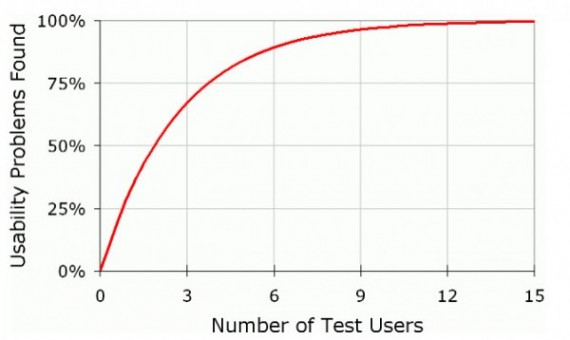
\includegraphics[scale=0.5]{Stichprobe.jpg}
	\caption{Stichprobengröße für Usability Tests}
	\label{fig2}
\end{figure}
\newpage
\section{Vorbereitung}
Für uns war es besonders wichtig zu sehen, ob Probanden die für sie unbekannte App, mühelos bedienen können und problemlos die vorgegebenen Ziele erreichen können.
Generelles Feedback, z.b. der Wunsch nach weiteren Funktionalitäten, war im Hinblick auf eine eventuelle Veröffentlichung der Applikation ebenfalls interessant für uns. \\
Unter diesen Gesichtspunkten haben wir folgendne Fragebogen (Abbilding 5.2) zusammengestellt, den die Probanden, nach Durchführung von festgelegten Aufgaben(Listing 5.1.), ausfüllen durften.\\
Um sicherzustellen, dass unsere Aufgaben und Befragung nicht zu viel Zeit in Anspruch nehmen, haben wir es vorher selbst durchgespielt und uns dabei bewusst Zeit gelassen.



\subsubsection*{Listing 5.1. Aufgabenliste}
\begin{itemize}
	\item 1.) Bearbeite dein Profil: Ändere den Namen und das Profilbild
	\item 2.) Plane zwischen 12 und 14 Uhr an der Cafeteria Essen zu gehen
	\item 3.) Trete einer Gruppe bei
	\item 4.) Schau dir das Profil eines Gruppenmitgliedes an
	\item 5.) Verlasse die Gruppe
	\item 6.) Erstelle eine eigene Gruppe
\end{itemize}
\newpage
\begin{figure}[H]
	\centering
  \includegraphics[scale=0.7]{Umfrage.pdf}
	\caption{Evaluationsbogen}
	\label{fig2}
\end{figure}
\newpage

\section{Durchführung}
Es wurden Personen auf dem KIT Campus, welche im Forum saßen, folgendermaßen angesprochen: \\
\ \\
\textit{Hallo, dürfen wir euch eine Frage stellen? Esst ihr regelmäßig in der Mensa?} \\ 
\ \\
Personen die diese Frage bejahten kamen als Probanden in Frage. \\
\ \\
\textit{Würdet ihr an einer kleinen Umfrage teilnehmen, es dauert nur 5 Minuten und als Dankeschön bekommt ihr ein paar Schoko Bons.}  \\ 
\ \\
Bei Zusage wurde eine Person aus der Personengruppe ausgewählt.\\
\ \\
\textit{Also, wir haben eine App entwickelt, mit der sich Leute anonym mit Fremden zum Essen gehen an der Mensa verabreden können und wir wollten uns etwas Feedback dazu einholen, deshalb darfst du die App jetzt kurz für uns testen. Du kriegst gleich ein Handy von uns, auf dem ist bereits ein User registriert und eingeloggt und dann musst du einfach diese sechs Aufgaben(zeigt Aufgabenliste) abarbeiten.} \\
\ \\
Während der Durchführung achteten wir auf die Zeit, schauten aufmerksam zu und notierten uns hinterher unsere Beobachtungen, die im Abschnitt Ergebnisse aufgeführt sind. \\
Nachdem die Aufgaben durchgeführt wurden erhielten die Probanden den Evaluatiosbogen.\\
\ \\
\textit{So, du hast jetzt während den Aufgaben alle Funktionalitäten der App kennen gelernt, jetzt musst du nur noch diesen Umfragebogen ausfüllen und dann bist du fertig.}

\newpage
\section{Ergebnisse}
Unser Test umfasste sieben Probanden, die alle auf oben beschriebene Weise am Campus angesprochen wurden.

\subsection*{Beobachtungen}
Die Probanden benötigten jeweils 5-7 Minuten für den gesamten Test, ab dem Zeitpunkt, ab dem sie das Handy und die Aufgabenliste bekamen. Hauptsächlich nahmen sie sich unterschiedlich viel Zeit für den Fragebogen.\\
\ \\
Zwei Probanden speicherten ihre Profiländerung nicht über den Speichern-Button sondern drückten stattdessen auf Zurück  um wieder in das Home Menü zu gelangen.
\ \\
Sechs von sieben Probanden haben nicht gemerkt, dass nicht nur drei sondern sechs Proflbilder zur Wahl standen.
\ \\
Beim Erstellen einer Gruppe ist die maximale Mitgliederzahl auf 1 einstellbar. 

\subsection*{Auswertung der Evaluationsbögen}
\ \\
\begin{tikzpicture}\begin{axis}[width=1.1\textwidth,height=0.6\textwidth,ybar,enlargelimits=0.1,symbolic x coords={Trifft nicht zu, Trifft eher nicht zu, Neutral, Trifft eher zu, Trifft voll zu}
,xtick={Trifft nicht zu, Trifft eher nicht zu, Neutral, Trifft eher zu, Trifft voll zu}, ylabel={Anzahl Antworten}]

\addplot[color=blue] coordinates{(Trifft nicht zu,0) (Trifft eher nicht zu,0) (Neutral,0) (Trifft eher zu,2) (Trifft voll zu,5)};
\addplot[color=red] coordinates{(Trifft nicht zu,1) (Trifft eher nicht zu,2) (Neutral,1) (Trifft eher zu,1) (Trifft voll zu,2)};
\addplot[color=green] coordinates{(Trifft nicht zu,0) (Trifft eher nicht zu,0) (Neutral,0) (Trifft eher zu,1) (Trifft voll zu,6)};

\end{axis} 
\end{tikzpicture}
\ \\
Legende: \ \\
Blau: Die App war intuitiv/leicht bedienbar. \\
Rot:  Ich würde diese App selber benutzen/weiterempfehlen. \\
Grün: Das Design hat mir gefallen.

\newpage
\subsection*{Antworten in den Freitextfeldern}

\subsubsection*{Wünscht du dir noch weitere Funktionen?}
Vier von sieben Probanden füllten dieses Feld aus: \\
\ \\
- Hashtags für die Gruppen zum Suchen \\
- Bewertungssystem für das Essen \\
- Aktualisieren des Essenplans, wenn etwas ausgegangen ist \\ 
- Bewerten von Essen und Personen \\
- Chat innerhalb der Gruppe

\subsubsection*{Was hat dir gefallen, was hat dir nicht gefallen?}
Zwei von sieben Probanden füllten dieses Feld aus: \\
\ \\
- Einfache Bedienbarkeit, Gute Funktionalität und vorrausschauendes Texting \\
- Hübsches Design \\
\ \\
\subsection*{Fazit}

TODO


\printglossaries
\end{document}